\documentclass[a4paper,14pt]{extarticle}

\usepackage{ntv}
\usepackage{amsmath,amssymb}
\usepackage{float}
\usepackage{graphicx}
\usepackage{csquotes}
\usepackage[
  backend=biber,
  style=gost-numeric,
  sorting=none,
  giveninits=true
]{biblatex}
\addbibresource{references.bib}
\usepackage{hyperref}
\graphicspath{{./}{../assets/}{assets/}}

\title{Название статьи на русском языке}
\author{Иванов И. И.\textsuperscript{1}, Петров П. П.\textsuperscript{1, 2}}
\date{}

\begin{document}

\noindent УДК 000.000

\maketitle

\begin{center}
\textit{\textsuperscript{1}Университет, Санкт-Петербург, 000000, Россия}\\
\textit{\textsuperscript{2}Организация, Москва, 000000, Россия}\\
\textit{author@example.org}
\end{center}
\vspace{-9pt}

\textbf{Аннотация.} Здесь размещается аннотация статьи. Она должна кратко
описывать постановку задачи, используемый метод, основные результаты и выводы.
Для DOCX этот абзац автоматически получает стиль  аннотации из  журнального
шаблона. 

\noindent\textit{\textbf{Ключевые слова:} первое понятие, второе понятие,
третье понятие}

\vspace{4pt}
\begin{center}
\textbf{English Article Title}
\end{center}

\begin{center}
Ivanov I. I.\textsuperscript{1}, Petrov P. P.\textsuperscript{1, 2}\\
\textit{\textsuperscript{1}University, Saint Petersburg, Russia}\\
\textit{\textsuperscript{2}Organization, Moscow, Russia}\\
\textit{author@example.org}
\end{center}
\vspace{-6pt}

\textbf{Abstract.} Place the English abstract here. It should state the problem,
method, principal results, and conclusions without references to the main text.

\noindent\textit{\textbf{Keywords:} first concept, second concept, third concept}

\paragraph*{Введение} Основной текст набирается обычными абзацами. Заголовки
разделов в исходном документе являются полужирными заголовками в начале
абзаца, поэтому для них используется команда \verb|\paragraph*{...}|.
Ссылки на источники создаются из библиографической базы командой
\verb|\cite|~\cite{ivanov2026}.

Следующий абзац показывает стандартный отступ первой строки, выравнивание по
ширине и межстрочный интервал. Произвольные команды, зависящие от движка
TeX, могут не иметь прямого аналога в Word; для переносимого результата
предпочтительны стандартные структуры LaTeX~\cite{author2025}.



\paragraph*{Математическая модель} Формулы набираются средствами
\texttt{amsmath}. Номер можно зафиксировать командой \verb|\tag|, если он
должен совпадать в PDF и DOCX:
\begin{equation}
  E = \frac{F L^3}{48 I \delta}.
  \tag{1}
\end{equation}
где $E$~--- модуль Юнга, $F$~--- сила, $L$~--- длина образца,
$I$~--- момент инерции, $\delta$~--- перемещение.

\begin{figure}[H]
  \centering
  \vspace{7pt}
  % Replace this bundled sample with a project image under assets/.
  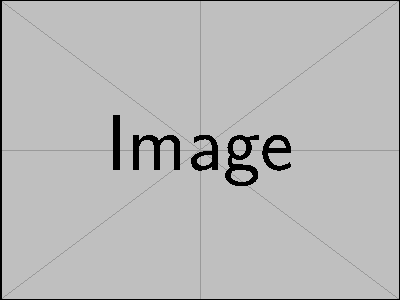
\includegraphics[width=0.80\textwidth]{../assets/example-image.png}
  \caption{Пример оформления рисунка}
  \label{fig:example}
\end{figure}
\vspace{-7pt}

Я пишу туту текст, который будет отображаться в PDF и DOCX. В Word. Формулы можно вставить в текст \(x^2 + y^2 = \text{радиус}^2\) и даже на русском языке если очень хочется. ООо это что латех приборы

\begin{table}[H]
  % Keep the caption above the tabular environment for the NTV layout.
  \centering
  \caption{Пример оформления таблицы}
  \label{tab:parameters}
  {\fontsize{14}{18}\selectfont
  \setlength{\tabcolsep}{34.5pt}
  \begin{tabular}{|l|c|c|}
    \hline
    Параметр & Обозначение & Значение \\
    \hline
    Длина & \textit{L} & 70 мм \\
    \hline
    Ширина & \textit{b} & 35 мм \\
    \hline
  \end{tabular}}
\end{table}
\vspace{-10pt}

Результаты показаны на рисунке~\ref{fig:example}, а исходные параметры
приведены в таблице~\ref{tab:parameters}.

\newpage
\section*{Список литературы}
\printbibliography[heading=none]

\newpage
\section*{СВЕДЕНИЯ ОБ АВТОРАХ}

Фамилия: Иванов

Имя: Иван

Отчество: Иванович

Должность: инженер

Полное название организации: Университет

E-mail: author@example.org

\end{document}
